\documentclass{ltjsarticle}
\usepackage{graphicx}
\usepackage{listings}
\usepackage{url}
\usepackage{float}

% 表紙情報
\title{ミニPBL レポート}
\author{学生番号:1TE23035E\\氏名:平野健汰}
\date{\today}

\begin{document}
\maketitle
\tableofcontents
\newpage

\section{課題の説明}
今回作成したのは,ゲームなどでよくあるガチャシステムである.
ユーザはガチャを引くことで,アイテムを入手することができる.
アイテムはレアリティによって分類され,レアリティが高いほど入手確率が低い.

\section{要求分析}
\subsection{機能要件}
\begin{itemize}
  \item 必須要件
  \begin{itemize}
    \item ユーザーがガチャを引ける機能
    \item ユーザーが引いたカードを確認できる機能
    \item ユーザーがアカウントにログインできる機能
    \item 運営がカードを登録できる機能
    \item 運営がガチャテーブルを設定できる機能
  \end{itemize}
  \item 追加要件
  \begin{itemize}
    \item ユーザーが引いたカードを検索できる機能
    \item ユーザーがゲーム内通過を用いて直接カードを入手できる機能
    \item ユーザーがガチャの内容を確認できる
  \end{itemize}
\end{itemize}

\subsection{ユースケース図}
今回作成したユースケース図は機能要件をそのまま表現している.
\begin{figure}[H]
    \centering
    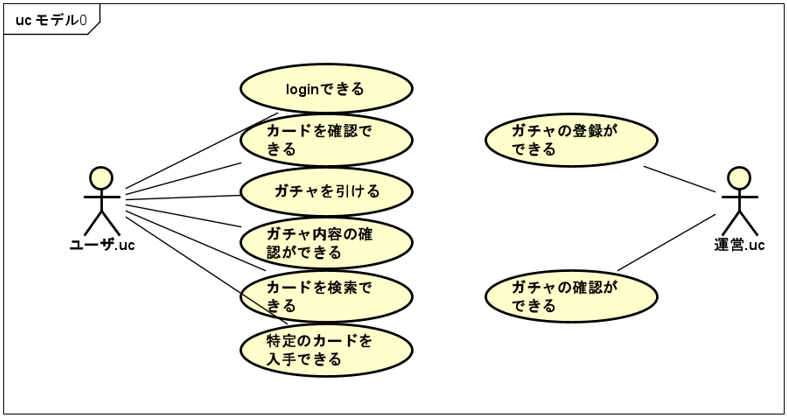
\includegraphics[width=0.8\textwidth]{src/usecase.png}
    \caption{ユースケース図}
    \label{fig:usecase}
\end{figure}

\subsection{ドメインモデル図}
今回作成したドメインモデル図は,ユーザ,カード,ガチャテーブル,運営の4つのクラスを持っている.
カードはガチャテーブルを参照することができる.
ガチャテーブルは運営によって設定される.
運営はカードを登録・削除することができる.
\begin{figure}[H]
    \centering
    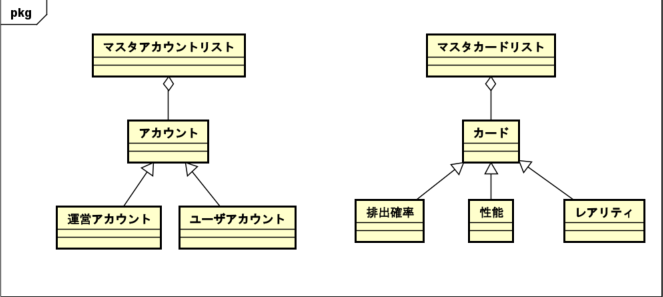
\includegraphics[width=0.8\textwidth]{src/domainModel.png}
    \caption{ドメインモデル図}
    \label{fig:domain}
\end{figure}

\section{オブジェクト指向分析/設計}
今回私が作製したのは,ログイン機能,サインアップ機能,カードの確認機能である.

\subsection{ユースケース記述}
想定通りの動きをしてくれる基本コースと,想定外の動きをした場合の代替コースを記述する.
\subsubsection{ログイン機能}
\begin{itemize}
  \item 基本コース
  \begin{itemize}
    \item ユーザはログイン・サインアップリンクをクリックする
    \item システムはログイン・サインアップページを表示する
    \item ユーザはユーザIDとパスワードを入力する
    \item システムはバリデーションを行う
    \item システムはハッシュ化したパスワードとユーザIDをデータベースと照合する
    \item システムはユーザを認証する
    \item システムはホーム画面を表示する
  \end{itemize}
  \item 代替コース
  \begin{itemize}
    \item ユーザIDまたはパスワードが間違っている場合
    \begin{itemize}
      \item システムはエラーメッセージを表示する
      \item ユーザは再度ユーザIDとパスワードを入力する
    \end{itemize}
  \end{itemize}
\end{itemize}

\subsubsection{サインアップ機能}
\begin{itemize}
  \item 基本コース
  \begin{itemize}
    \item ユーザはログイン・サインアップリンクをクリックする
    \item システムはログイン・サインアップページを表示する
    \item ユーザはユーザIDとパスワードを入力する
    \item システムはバリデーションを行う
    \item システムはユーザIDとパスワードをデータベースに登録する
    \item システムはユーザを認証する
    \item システムはホーム画面を表示する
  \end{itemize}
  \item 代替コース
  \begin{itemize}
    \item ユーザIDが既に登録されている場合
    \begin{itemize}
      \item システムはエラーメッセージを表示する
      \item ユーザは再度ユーザIDとパスワードを入力する
    \end{itemize}
    \item ユーザIDまたはパスワードが短い場合
    \begin{itemize}
      \item システムはエラーメッセージを表示する
      \item ユーザは再度ユーザIDとパスワードを入力する
    \end{itemize}
  \end{itemize}
\end{itemize}

\subsubsection{カードの確認機能}
\begin{itemize}
  \item 基本コース
  \begin{itemize}
    \item ユーザはカード確認リンクをクリックする
    \item システムはカード確認ページを表示する
    \item システムはユーザが引いたカードを表示する
  \end{itemize}
\end{itemize}

班員は,ガチャを引く機能,ガチャ内容を確認できる機能,カードの検索機能,ガチャ登録機能,ガチャ確認機能を作製した.

\subsection{ロバストネス図}
ユースケース記述をもとに,ロバストネス図を作製した.
画面を表すバウンダリ,オブジェクトを表すエンティティ,アクションを表すコントロールを配置した.
\subsubsection{ログイン機能}
\begin{figure}[H]
    \centering
    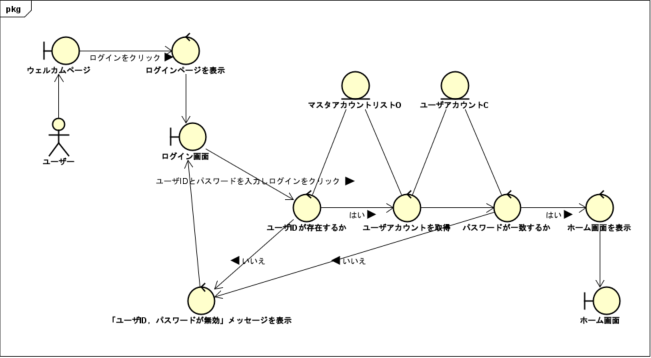
\includegraphics[width=0.8\textwidth]{src/loginRobustness.png}
    \caption{ログイン機能のロバストネス図}
    \label{fig:robustnessLogin}
\end{figure}

\subsubsection{サインアップ機能}
\begin{figure}[H]
    \centering
    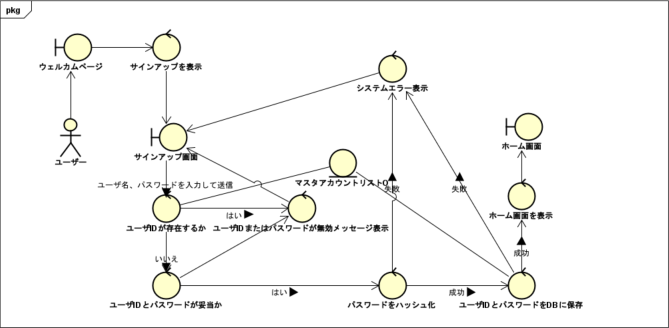
\includegraphics[width=0.8\textwidth]{src/signupRobustness.png}
    \caption{サインアップ機能のロバストネス図}
    \label{fig:robustnessSignup}
\end{figure}

\subsubsection{カードの確認機能}
\begin{figure}[H]
    \centering
    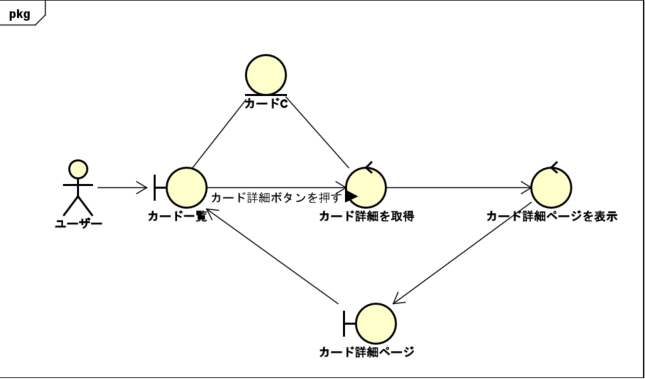
\includegraphics[width=0.8\textwidth]{src/cardRobustness.png}
    \caption{カードの確認機能のロバストネス図}
    \label{fig:robustnessCard}
\end{figure}

班員は,ガチャを引く機能,ガチャ内容を確認できる機能,カードの検索機能,ガチャ登録機能,ガチャ確認機能を作製した.

\subsection{シーケンス図}
ロバストネス図をもとに,シーケンス図を作製した.
クラスの責務を割り当てることを目的に作製した.

\subsubsection{ログイン機能}
\begin{figure}[H]
    \centering
    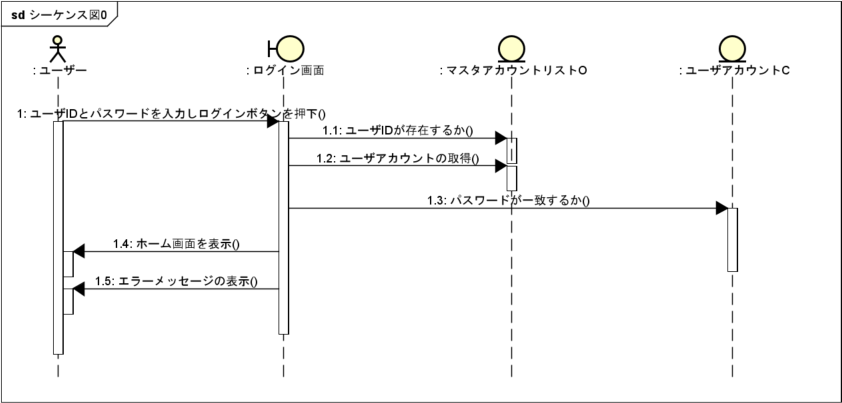
\includegraphics[width=0.8\textwidth]{src/loginSequence.png}
    \caption{ログイン機能のシーケンス図}
    \label{fig:sequenceLogin}
\end{figure}

\subsubsection{サインアップ機能}
\begin{figure}[H]
    \centering
    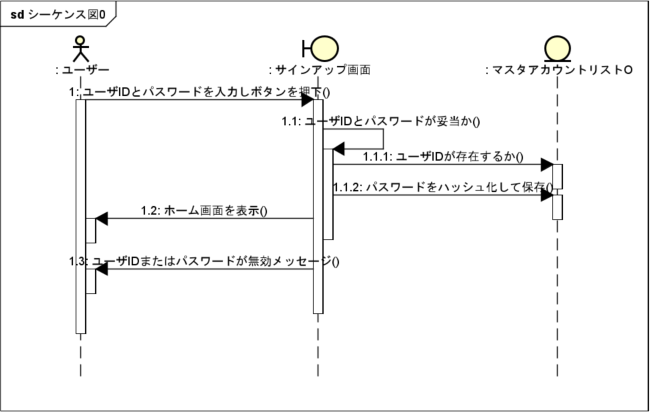
\includegraphics[width=0.8\textwidth]{src/signupSequence.png}
    \caption{サインアップ機能のシーケンス図}
    \label{fig:sequenceSignup}
\end{figure}

\subsubsection{カードの確認機能}
\begin{figure}[H]
    \centering
    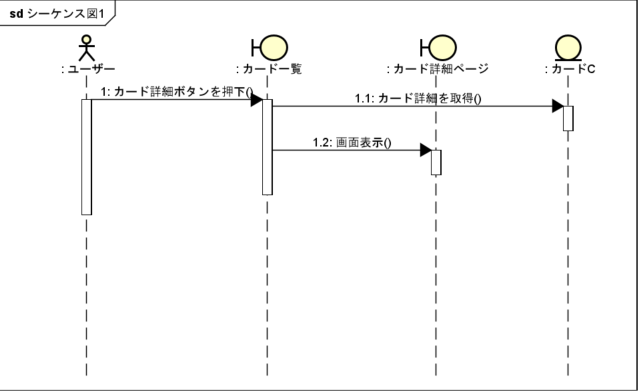
\includegraphics[width=0.8\textwidth]{src/cardSequence.png}
    \caption{カードの確認機能のシーケンス図}
    \label{fig:sequenceCard}
\end{figure}

\section{クラス図}
シーケンス図をもとに,クラス図を作製した.
目的はクラスの責務を構造化することである.
\begin{figure}[H]
    \centering
    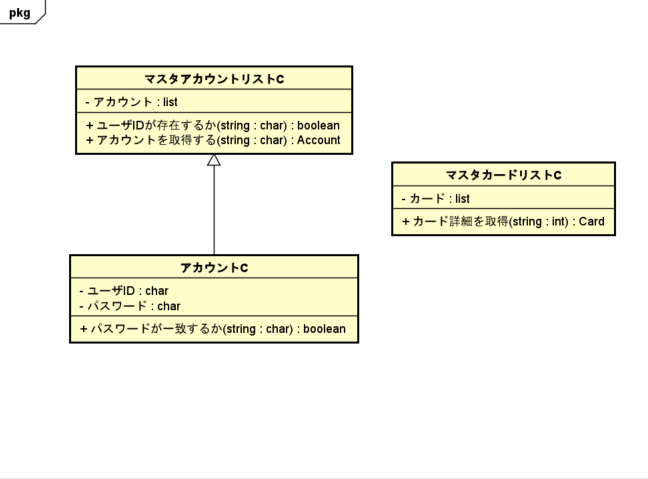
\includegraphics[width=0.8\textwidth]{src/class.png}
    \caption{クラス図}
    \label{fig:class}
\end{figure}

\section{実装コード(バックエンドの一部を抜粋)}
\subsection{バックエンド}
\begin{lstlisting}[frame=single, lineskip=-5pt]
// ログイン機能 
  CROW_ROUTE(app, "/login").methods(crow::HTTPMethod::POST)
  ([&](const crow::request &req)
  {
      auto body = crow::json::load(req.body);

      // JSONのキーが存在するか確認
      if (!body || !body.has("username") || !body.has("password"))
      {
          return crow::response(400, "Missing 'username', 'password'");
      }

      // username, passwordの取得
      std::string name = body["username"].s();
      std::string pass = body["password"].s();

      // ユーザー名とパスワードの組み合わせを確認
      int id = search_user_data(name, pass);
      if (id > 0 && id != 9999)
      {
          sessionCounter++;
          session[sessionCounter] = id; // sessionに保存
          // 正常にログインした場合、tokenとしてsessionCounterを返す
          return crow::response(crow::json::wvalue{
              {"status", "success"},
              {"token", sessionCounter}}); // ログイン成功
      }
      else if (id == 9999)
      {
          sessionCounter++;
          session[sessionCounter] = id; // sessionに保存
          // 正常にログインした場合、tokenとしてsessionCounterを返す
          return crow::response(crow::json::wvalue{
              {"status", "admin-success"},
              {"token", sessionCounter}}); // ログイン成功
      }
      return crow::response(409, "Username or Password is invalid"); 
      // ユーザー名またはパスワードが無効
  });
\end{lstlisting}

\section{考察}
今回私は上述した昨日のPBLを行った.
そして実装を行い,フロントエンド側を担当した.
フロントエンドはReact,バックエンドはC++で実装した.
今回のPBLを通して,オブジェクト指向の設計を行うことの重要性を学んだ.
今回のPBL,実装を通して,設計の重要性を確認すると同時に実装を考えずに設計を進めることは難しいと感じた.
これは設計の甘さのことであり,設計書が全くないよりは実装をやりやすいと感じたが,設計書以外の部分で考えなくてはならないことが多く,実装を考えながら設計を進めることの重要性を感じた.
上述したこれらのことは経験を積むことで解決することができると感じた.

\end{document}